
\begin{document}
\chapter{Method}
\section{Simulation of data}\label{ch:simulationOfData}
Simulations of data are performed in order to verify the theoretical behaviour of the models under the influence of different noise levels. The global position estimator is verified for the influence on the position and clock bias estimates where noise levels of growing magnitude is introduced. The relative position estimate is also simulated and compared between two global position and the DD estimator, which will be compared to the result of the observations.

\subsection{Testing different error sources impact on global position}\label{simNoiseConvergence}
The global positioning estimator's behaviour is tested using simulated data to verify the theoretical behaviour of the estimator. The simulations are based on creating pseudorange measurements between a stationary point on earth and corrupting it with noise, where actual receiver positions are used, and satellites are positioned according to the orbits from the data contained in the ephemeris messages. 
\par 
The simulations are performed and evaluated in two ways:
\begin{itemize}
\item The convergence of the receiver state estimates for an error of growing magnitude.
\item The trend of error in final state estimates for a noise of increasing magnitude.
\end{itemize} 
The noise types introduced are as follows:
\begin{itemize}
\item Initial position estimate error
\item Receiver clock bias
\item Satellite position random noise
\item Measurement white noise
\item Initial position and clock bias
\end{itemize}
Simulations of the initial estimate is simulated by setting the initial estimate ${\boldsymbol \theta}_0$ to be the sum of the true state ${\boldsymbol \theta}$ and a random noise ${\boldsymbol \epsilon}_p$. ${\boldsymbol \epsilon}_p$ is a $3\times1$ vector of Gaussian white noise, multiplied by a factor of increasing magnitude% from 10 to $10^7$ m.  
When simulating a receiver clock bias, one random value is added to all observation. Satellite position random noise is simulated by introducing errors in all the satellite positions. 
\par
For a simulation with initial estimate error, as well as a receiver clock bias, the position estimate is expected to converge to zero with numerical precision. A combination of receiver clock bias and initial position estimate is also expected to converge to zero. When a random noise is added to the satellite position or observations, the estimate error is expected to grow at the same rate as that of the noise. From the simulations, the impact of different noise sources on the estimate can be the analysed and used to identify potential errors in the estimation method. 

\subsection{RMSE of relative position from global position and DD estimate }\label{RMSE}
Since the DD-method has been shown to improve the relative estimate as mentioned in section \ref{previousResearch}, the hypothesis is that the DD-method is superior to that of two individual global fixes in mitigating the effect of a common noise. The behaviour is simulated using increasing levels of bias. This means that any two simulated observations between a satellite and the receivers will be of the form 
\begin{align}
y_a&=||{\bf p}^{(i)}-{\bf p}_{a}||+c\Delta t_a+\eta^{(i)}+ \epsilon_a\\
y_b&=||{\bf p}^{(i)}-{\bf p}_{b}||+c\Delta t_b+\eta^{(i)}+\epsilon_b.
\end{align}
The notation is consistent with that in section \ref{diffObsModel}. In the simulations, the shared non-white noise $\eta^{(i)}$ is randomly sampled and will be constant per satellite for the observation series. This is a simplification, as the common noise is assumed slow changing. The simulations are performed using increasing magnitudes for the bias level. The result is then presented as the root mean square error (RMSE) of the estimate, defined as
\begin{align}
e_{RMS}	&=\sqrt{\sum   |{\bf d-\hat{d}}|/n} \nonumber \\
		&=\sqrt{\frac{1}{n}\sum_{i=k}^{n} ({\bf d-\hat{d}}[k])\cdot ({\bf d-\hat{d}}[k])^T} \label{eqERMS}
\end{align} 
for a true baseline vector $\bf d$ and the corresponding estimated distance ${\bf \hat{d}}[k]$ for an epoch $k$. Since the experiment is conducted using the north and east direction separation, the baseline vector will be set to respectively $[10, 0,0]$ m and $[0, 10, 0]$ m.


\section{GNSS positioning from observation data}

\subsection{Data extraction from sensor}
The INS unit allows for data sampling and streaming in real-time as well as logging for post-processing through three different types of software. A GUI called EvalTool is available from the producer Inertial Sense\footnote{\url{https://docs.inertialsense.com/user-manual/software/evaltool/}} for logging data for most applications, both fused and unfused data from the GNSS-receiver and the IMU units. In addition to that, there is a command-line tool called CL Tool for logging of much the same functionality\footnote{\url{https://docs.inertialsense.com/user-manual/software/cltool/}}. However, for the sake of this project, unprocessed pseudorange observation data from the receivers were required to implement and compare the single and double-difference methods described in chapter \ref{RelPos}. In order to extract those, data must be parsed directly from the Software Development Kit (SDK) projects available. A logger, producing comma-separated values (.csv)-type log files of the received packages is available at \url{https://github.com/Kallemange/Communications} for post-processing. More information on the logger and data structures in use can be found in appendix \ref{structsAndLogs}.
\subsection{Experimental setup}\label{experimentalSetup}
In order to test the receiver's behavior over time, two receivers are placed stationary at a baseline of 10 m pointing first in N-direction as well as in E-direction, with measurements taken for approximately 30 minutes in Uggleviksk\"allan, a glade in the forest on coordinates: 59.353$^o$N, 18.073$^o$E, shown in figure \ref{fig:Uggleviken}. One receiver was placed close to the pin indicated in the figure, and the other positioned east and south of it.
\begin{figure}[!h]
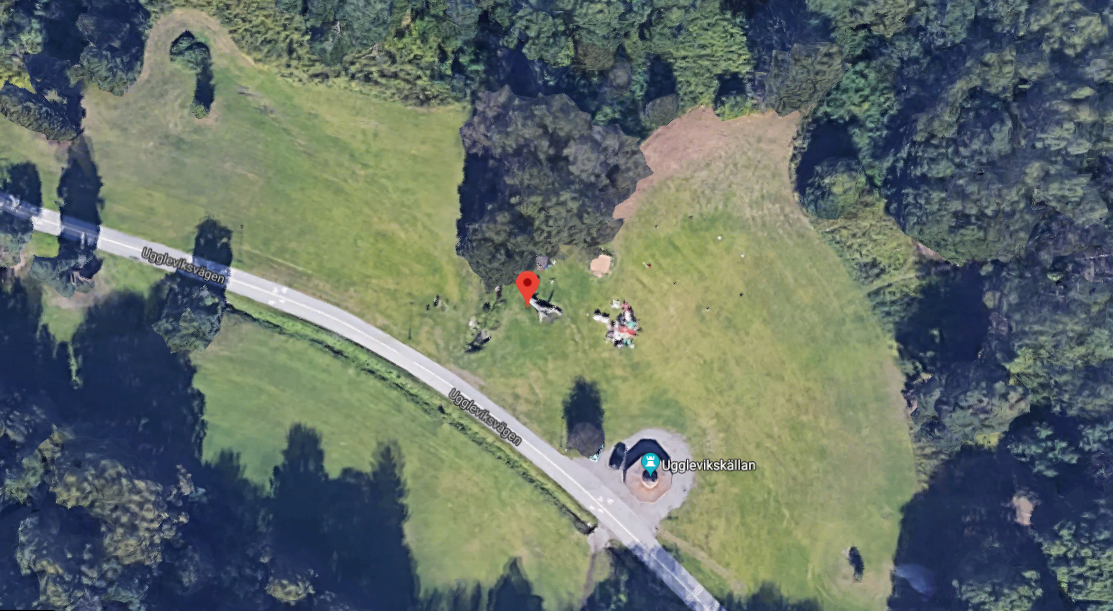
\includegraphics[scale=0.4]{Method/Uggleviken}
\caption{\label{fig:Uggleviken} Uggleviken, place where observations were made. Image taken from Google Maps: \url{https://www.google.com/maps}}
\end{figure} 
The directions were set using a 
digital compass on an android phone and the distance through using a measuring tape. The logger is started for the receivers separately, but are connected to the same computer where the log files are stored. 

%\subsection{Estimating satellite position}
%To verify that the satellite trajectories are correct the satellite positions are calculated for a given time span using the method described in section \ref{chap:ephPositioning} from the received ephemeris data. This is then compared to the historical satellite positions available on-line\footnote{e.g. \url{https://in-the-sky.org/} and \url{https://www.gnssplanning.com/\# /charts}}. Plots showing the trajectory, as well as elevation and azimuth for a given time frame are produced and compared in section \ref{satelliteTrajectory}. 

\subsection{Global and relative positions from onboard estimate}
The onboard estimates are sampled and logged in parallel to the raw data. This contains information on the global position in an ECEF or LLA-frame, HDOP and VDOP values as well as sampling time. This data will be called the onboard estimate. From this, an estimate of the variance in each direction can be made.
\subsection{Global and relative position estimates from raw data}
The method for how the positioning is made in the individual as well as the relative case using the log files is presented in the following section. The solutions have only been implemented based on log files and are not made to run real-time.
The solution is calculated in two steps: 
\begin{enumerate}
\item Load the data from log files into an array with a struct for each epoch. 
\item Calculate the solution per epoch from the observation and ephemeris data
\end{enumerate} 
\subsubsection{Global positioning}
The positioning of each receiver only utilizes the ephemeris data collected by the same receiver and only observation data that has a corresponding ephemeris reading is used. The method for positioning which is implemented follows the description in section \ref{stateEst}. The solution is an instantaneous estimate for each epoch, indicating that the previous estimate is not taken into account for the current one. This will produce a solution calculated in an ECEF coordinate frame, which is then projected to a NED frame. The solution includes a global position, calculated as described in section \ref{globalWEstimator} with the weighted estimator of equation \ref{SNRWeights}, an estimate of the HDOP and VDOP values, as described in (\ref{eq:HDOP}-\ref{eq:VDOP}) as well as a variance over the solution, calculated per direction in a NED-frame.

\subsection{Double difference relative positioning}
For the DD relative positioning algorithm, the set of satellites from which the receivers have sampled observations must be equal each epoch. Any observation not present in both is discarded. 
%The position must always be calculated using one of the receivers, which will be called $r_a$, as reference. This means that the direction vectors to the satellites are calculated based on the estimate ${\bf p}_a$. 
This method, which follows the algorithm for double difference in section \ref{RelPos} utilizes that the clock error cancels out and will not be estimated. The satellite position is instead calculated at the nominal time of observation $t_{rec}$. This is due to the angular change, as opposed to the position change, between satellite and receiver is negligible within the time frame of a sample. 
\par
The relative position estimate also requires the receiver position ${\bf p}_a$, in order to calculate the unit vector ${\bf e}^i$ pointing to a satellite from a receiver. The receiver position used is that given by the onboard estimate. The system of equations is then solved for the given reference satellite, which will be selected as that with the highest SNR value for each epoch, as suggested in \cite{BLUE}. The solution will give an instantaneous relative positional estimate for r$_b$ with regards to r$_a$ in an ECEF frame, which is then projected down to a NED solution through the point given. Given that the receivers were stationary, the estimates are expressed as a mean and a standard deviation in each direction.

\end{document}
